\def\difficulty{1}
\sujet{Binary Mathematical Morphology}
\label{tut:binarymorpho:enonce}
\index{Mathematical Morphology}

\begin{note}The objective of this tutorial is to process binary images with the elementary operators of mathematical morphology. More particularly, different image transformations, based on the morphological reconstruction, will be studied (closing holes, removing small objects\dots).\end{note}

The different transformations will be applied on the following images Fig. \ref{fig:morpho:images}:
\begin{figure}[htbp]
\centering\caption{Images to use for this tutorial.}
\subfloat[$I_1$.]{{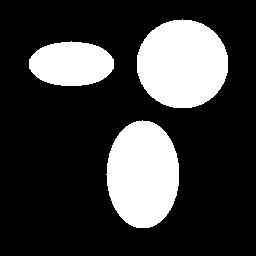
\includegraphics[width=3.25cm]{A.jpg}}}\hspace{.5cm}
\subfloat[$M$.]{{
\includegraphics[width=3.25cm]{M.jpg}}}\hspace{.5cm}
\subfloat[$I_2$.]{{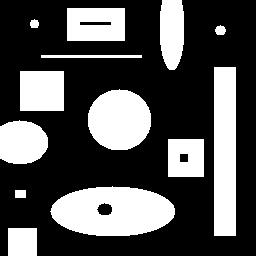
\includegraphics[width=3.25cm]{B.jpg}}}\hspace{.5cm}
\subfloat[Cells.]{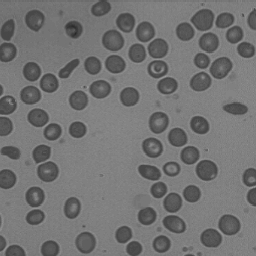
\includegraphics[width=3.25cm]{cells.jpg}\label{fig:morpho:images:cells}}%
 \label{fig:morpho:images}%
 \vspace*{-8pt}%
\end{figure}

\vspace*{-14pt}

\section{Introduction to mathematical mor\-pho\-lo\-gy}

Mathematical morphology started in the 1960s with Serra and Mathe\-ron \cite{Serra1982}. It is based on Minkowski addition of sets.  The main operators are erosion and dilation, and by composition, opening and closing. More informations can be found in \cite{Soille2003}.

The erosion of a binary set $A$ by the structuring element $B$ is defined by:
\begin{equation}\varepsilon_B (A)= A \ominus B = \{z\in A | B_{z} \subseteq A\}
\end{equation}

where, $B_z=\{b+z|b\in B\}$.

The dilation can by obtained by:
\begin{equation}\delta_B(A)=A  \oplus B = \{z \in A| (B^{s})_{z} \cap A\neq \varnothing\}\end{equation}
where $B^{s}=\{x\in E | -x \in B\}$ is the symmetric of $B$.

By composition, the opening is defined as:
$A \circ B  = (A \ominus B) \oplus B$.
The closing is defined as:
$A \bullet B  = (A \oplus B) \ominus B $.

\section{Elementary operators}
\index{Mathematical Morphology!Erosion}
\index{Mathematical Morphology!Dilation}
\begin{qbox}
Test the functions  of dilation, erosion, opening and closing on the image $I_2$ by varying:
\begin{enumerate}
	\item the shape of the structuring element,
	\item the size of the structuring element.
\end{enumerate}
\end{qbox}

\begin{mcomment}
\begin{mremark}
The \matlabregistered{} functions are \minline{imdilate}, \minline{imerode}, \minline{imopen} and \minline{imclose}. The func\-tion \minline{strel} creates a structuring element.
\end{mremark}
\end{mcomment}
\begin{pcomment}
\begin{premark}
The python functions come from the python module \pinline{scipy.ndimage.morphology}. Useful func\-tions are \pinline{binary_dilation}, \pinline{binary_erosion}, 
 \pinline{binary_opening} and
\pinline{binary_closing}.
 The function \pinline{ndimage.generate_binary_structure} creates a structuring element.
\end{premark}
\end{pcomment}

\section{Morphological reconstruction}\index{Mathematical Morphology!Reconstruction}
The operator of morphological reconstruction $\rho$ is very powerful and largely used for practical applications.
The principle is very simple. We consider two binary images: $I_1$ (the studied binary image) and $M$ (the marker image).
The objective is to reconstruct the elements of $I_1$ marked by $M$ as illustrated in the Fig. \ref{fig:morpho:reconstruction}.

To do this, we iteratively dilate the marker $M$ while being included in $I_1$ (see Eq.\ref{eq:binarymorpho:enonce:rho}).
In order to guarantee this inclusion in $A$, we keep from each dilated set its intersection with $I_1$.
The algorithm is stopped when the process dilation-intersection is equal to the identity transformation (convergence).

\begin{figure}[htbp]
\centering\caption{Illustration of morphological reconstruction of $I_1$ by $M$.}%
\subfloat[$I_1$]{{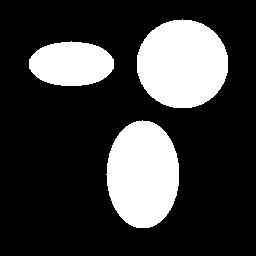
\includegraphics[width=3cm]{A.jpg}}}\hspace{.5cm}
\subfloat[$M$]{{
\includegraphics[width=3cm]{M.jpg}}}\hspace{.5cm}
\subfloat[$rec(I_1,M)$]{{
\includegraphics[width=3cm]{rec.jpg}}}%
\label{fig:morpho:reconstruction}%
\end{figure}

Let $\delta^c_I(M)= \delta_{B_1}(M) \cap I$ be the dilation of the marker set $M$ constrained to the set $I$. Then, the morphological reconstruction is defined as:
\begin{equation}\rho_I(M) = \lim_{n\rightarrow \infty} \underbrace{\delta_I \circ \ldots \circ \delta_I(M)}_{n \textrm{ times}}
 \label{eq:binarymorpho:enonce:rho}
\end{equation}



\begin{algorithm}[H]
\SetAlgoLined
\KwData{image $I$ and marker $M$}
\KwResult{reconstructed image $rec(I,M)$}
$r=area(M)$\;
$s=0$\;
\While{$r \neq s$}{
$s=r$\;
$M=I\cap (M\oplus B_1)$\;
$r=area(M)$\;
}
$rec(I,M)=M$\;
\caption{The algorithm of this morphological reconstruction}
\end{algorithm}

\begin{qbox}
\begin{enumerate}
\item Implement the algorithm.
\item Test this operator with the images $I_1$ and $M$.
\end{enumerate}
\end{qbox}

\begin{mcomment}

\begin{mremark}
The function \minline{bwarea} evaluates the area of a 2D binary object.
\end{mremark} 
\end{mcomment}

\begin{pcomment}
 \begin{premark}
  Evaluate the area of a set may be done  by counting the number of its pixels.
 \end{premark}

\end{pcomment}



\section{Operators by reconstruction}
\begin{qbox}
Using the reconstruction operator, implement the 3 following transformations:
\begin{enumerate}
   \item removing the border objects,
	\item removing the small objects,
	\item closing the object holes.
\end{enumerate}
Test these operators on the image $I_2$.
\end{qbox}

\begin{mcomment}
\begin{mremark}
The morphological reconstruction function to use is \minline{imreconstruct}.
\end{mremark}
\end{mcomment}

\begin{pcomment}
\begin{premark}
The morphological reconstruction function to use is 
\pinline{binary_propagation} in the module \pinline{ndimage.morphology}.
\end{premark}
\end{pcomment}


\section{Cleaning of the image of cells}
\begin{qbox}
\begin{enumerate}
\item Threshold the image of cells (Fig. \ref{fig:morpho:images:cells}).
\item Process the resulting binary image with the 3 cleaning processes of the previous question.
\end{enumerate}
\end{qbox}

